\documentclass{standalone}
\usepackage{graphicx}	
\usepackage{amssymb, amsmath}
\usepackage{color}

\usepackage{tikz}
\usetikzlibrary{arrows.meta, backgrounds, math}
\usepackage{pgfmath}

\definecolor{light}{RGB}{220, 188, 188}
\definecolor{mid}{RGB}{185, 124, 124}
\definecolor{dark}{RGB}{143, 39, 39}
\definecolor{highlight}{RGB}{180, 31, 180}
\definecolor{light_teal}{RGB}{107, 142, 142}
\definecolor{mid_teal}{RGB}{72, 117, 117}
\definecolor{dark_teal}{RGB}{29, 79, 79}
\definecolor{gray10}{gray}{0.1}
\definecolor{gray20}{gray}{0.2}
\definecolor{gray30}{gray}{0.3}
\definecolor{gray40}{gray}{0.4}
\definecolor{gray60}{gray}{0.6}
\definecolor{gray70}{gray}{0.7}
\definecolor{gray80}{gray}{0.8}
\definecolor{gray90}{gray}{0.9}
\definecolor{gray95}{gray}{0.95}

\begin{document}

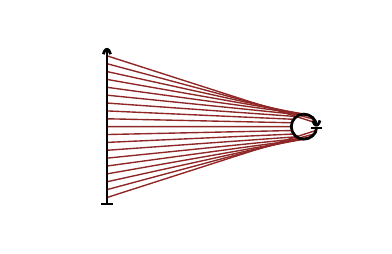
\begin{tikzpicture}[scale=1.0]

  \draw[white] (-1, -1.25) rectangle (3.25, 1.25);

  \pgfmathsetmacro{\r}{0.159154943091895}

  \foreach \y in {-0.9, -0.8, ..., 0.9} {
    \pgfmathsetmacro{\theta}{- (1 - \y) * 180};
    \pgfmathsetmacro{\xf}{2.5 + \r * cos(\theta)};
    \pgfmathsetmacro{\yf}{-\r * sin(\theta)};
    \draw[dark, line width=0.5] (0, \y) -- (\xf, \yf);
  }
  
  \begin{scope}[shift={(0, 0)}]
    \draw[{|[width=4]}-{Parenthesis[width=4]}, line width=1] (0, -1) -- (0, 1);
  \end{scope}
  
  \begin{scope}[shift={(2.5, 0)}]
    \draw[{|[width=4]}-{Parenthesis[width=4]}, line width=1] 
      (0:\r) arc (0:-360:\r);
  \end{scope}
  

\end{tikzpicture}

\end{document}  